\documentclass{article}
\usepackage[margin=1in]{geometry}
\usepackage{amsmath, amssymb, tikz, pgfplots}
\usetikzlibrary{positioning}

\title{\vspace{-3ex}Advanced Function Notes}
\author{Jeffrey Gao\and More Contributors Later}
\renewcommand\thesubsubsection{\thesubsection{} \Alph{subsubsection}}
\renewcommand\labelitemi{--}

\begin{document}
	\maketitle
	
	\section{Unit 1}
	\subsection{Functions}
	\subsubsection{Relations}
	A (binary) relation is defined as a set of ordered pairs $(x, y)$.
	A relation can be described using:
	\begin{itemize}
		\item words
		\item graphs
		\item equations
		\item inequalities
		\item lists of ordered pairs
		\item mapping diagrams
	\end{itemize}
	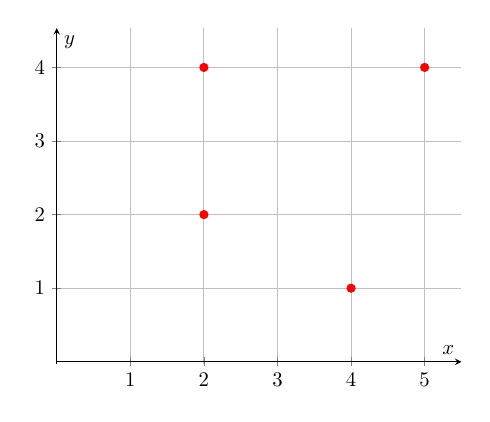
\begin{tikzpicture}[scale=.75]
		\begin{axis}[
			scatter/classes={a={draw=red,fill=red}},
			axis y line*=left,
			axis x line*=bottom,
			grid=both,
			ymin=0,
			xmin=0,
			ymax=4.5,
			xmax=5.5,
			axis equal,
			axis lines=middle,
			xlabel=$x$,
			ylabel=$y$
		]
		\addplot[scatter,only marks,scatter src=explicit symbolic]
		table[meta=label] {
			x y label
			2 2 a
			2 4 a
			4 1 a
			5 4 a
		};
		\end{axis}
	\end{tikzpicture}\\
	This relation as a set of ordered pairs is $R=\{(2, 2), (2, 4), (4, 1),(5, 4)\}$
	\subsubsection{Domain and Range of a Function}
	The domain of a relation is the set of all the x values such that the ordered pair $(x, y)$ satisfies (is an element of) the relation. The range of a relation is the set of all the y values such that the ordered pair $(x, y)$ satisfies (is an element of) the relation.\\\\
	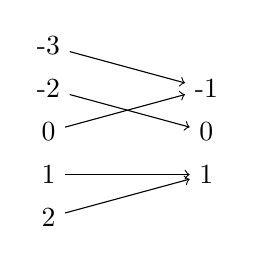
\begin{tikzpicture}[scale=.5]
		\node (n3) {-3};
		\node[below=2pt of n3] (n2) {-2};
		\node[below=2pt of n2] (o) {0};
		\node[below=2pt of o] (p1) {1};
		\node[below=2pt of p1] (p2) {2};
		
		\node[right=45pt of o] (o2) {0};
		\node[above=2pt of o2] (nn1) {-1};
		\node[below=2pt of o2] (pp1) {1};
		
		\draw[->] (n3) -- (nn1);
		\draw[->] (n2) -- (o2);
		\draw[->] (o) -- (nn1);
		\draw[->] (p1) -- (pp1);
		\draw[->] (p2) -- (pp1);
	\end{tikzpicture}
	For this mapping diagram, the domain would be $D=\{-3, -2, 0, 1, 2\}$ and the range would be $R=\{-1, 0, 1\}$
	\subsubsection{Functions}
	A function can only assign one element from the set of Y values (the range) to each element from the set of X values (the domain). $y=f(x)$ where $x$ is the argument or the input of the function and $y$ is the value or the output of the function.\\
	Using the function $f(x)=(x-1)^2$:
	\begin{itemize}
		\item $f(0)=1$
		\item $f(\frac{1}{2})=\frac{1}{4}$
		\item $f(a+2)=a^2+2a+1$
	\end{itemize}
	\subsection{Graph}
	The graph of a function $f$ is the graph of the set of ordered pairs $(x, y)$ where $y=f(x)$.\\
	The graph of the function defined a set of ordered pairs $f=\{(2, 3), (0, -2), (-4, 3), (4, 0), (-3, -3)\}$\\
	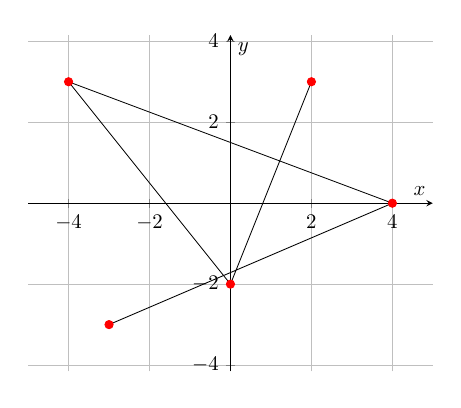
\begin{tikzpicture}[scale=.75]
		\begin{axis}[
			scatter/classes={a={draw=red,fill=red}},
			axis y line*=left,
			axis x line*=bottom,
			grid=both,
			ymin=-4,
			xmin=-5,
			ymax=4,
			xmax=5,
			axis equal,
			axis lines=middle,
			xlabel=$x$,
			ylabel=$y$
		]
		\addplot[scatter,scatter src=explicit symbolic]
		table[meta=label] {
			x y label
			2 3 a
			0 -2 a
			-4 3 a
			4 0 a
			-3 -3 a
		};
		\end{axis}
	\end{tikzpicture}\\
\end{document}